\documentclass{standalone}
\usepackage{tikz}
\usetikzlibrary{graphs,positioning}
\begin{document}
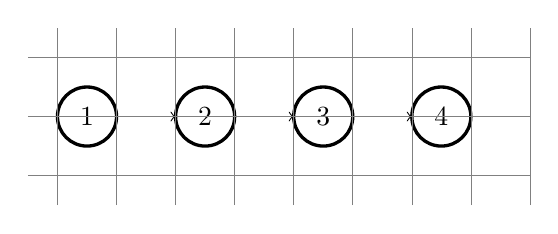
\begin{tikzpicture}[scale=0.75,
  every node/.style = {
    circle,
    very thick,
    inner sep = 0,
    outer sep = 0,
    minimum size = 0.75cm,
    draw = black,
    scale = 1,
  },
]
\graph[grow right sep = 5mm]{
  1 -> 2 -> 3 -> 4
};
\draw[help lines] (-0.5, -1.5) grid (8, 1.5);
\end{tikzpicture}
\end{document}

% I would like the following 10mm nodes to be fitting a 10mm grid using the `graph` command. Instead, the thickness is adding up (I would like TikZ to ignore it).

% [![misaligned nodes][1]][1]

%     \documentclass{standalone}
%     \usepackage{tikz}
%     \usetikzlibrary{graphs,positioning}
%     \begin{document}
%     \begin{tikzpicture}[
%       every node/.style = {
%         circle,
%         very thick,
%         inner sep = 0,
%         minimum size = 10mm,
%         draw = black,
%       },
%     ]
%     \graph[grow right sep=10mm]{
%       1 -> 2 -> 3 -> 4
%     };
%     \draw[help lines] (-0.5,-1.5) grid (8,1.5);
%     \end{tikzpicture}
%     \end{document}

% Am I supposed to size my nodes 10mm − "very thick"??? Sounds a little insane.


%   [1]: https://i.imgur.com/xLLP1ZZ.png